\appendix
% remove header trickery
\chapter[]{Anhang}
\section{Ergänzendes zum Experiment}
\addcontentsline{toc}{chapter}{A\ \ Anhang}
\begin{table}[H]
    \caption{Spannungswerte bei der Konditionierung}
    \label{tab:Konditionierung}
    \begin{tabular}{cccc}
        Spannungsdifferenz in V & Strom in mA &	Widerstand in M$\Omega$ & Zeitintervall in min\\   
        \midrule
            880  & 0,018 & 48,9 & 05:57\\
            980  & 0,021 & 46,7 & 06:39\\
            1080 & 0,024 & 45,0 & 05:36\\
            1200 & 0,028 & 42,9 & 07:26\\
            1330 & 0,032 & 41,6 & 07:20\\
            1450 & 0,036 & 40,3 & 04:13\\
            1580 & 0,040 & 39,5 & 04:41\\
            1700 & 0,044 & 38,6 & 04:43\\
            1825 & 0,048 & 38,0 & 06:01\\
            1940 & 0,052 & 37,3 & 05:10\\
            2060 & 0,056 & 36,8 & 07:45\\
            2160 & 0,059 & 36,6 & 05:57\\
            2270 & 0,063 & 36,0 & 05:59\\
            2380 & 0,068 & 35,0 & 06:16\\
            2480 & 0,071 & 34,9 & 06:27\\
            2600 & 0,071 & 36,6 & 06:02\\
            2700 & 0,080 & 33,8 & 06:46\\      
    \end{tabular}
\end{table}

\section{Herleitung zur Fehlerfortpflanzung}
\label{sec:fehlerfortpflanzung}
Damit die Herleitung der Fehlerfortpflanzung nachvollziehbar ist, wird im Folgenden die integrierten Counts (Fläche) der Peaks als $N_\text{peak}(\text{Ar}^{q+})$ als $N$ bezeichnet. Die Fläche des größten Peaks $N_\text{peak}(\text{Ar}^{+})$ wird als $G$ bezeichnet. Die normierte Fläche des Peaks $N_\text{peak, norm}(\text{Ar}^{q+})$ wird durch $N'$ dargestellt. 
\begin{equation}
    N' = \frac{N}{G} \cdot \sigma_+(E).
\end{equation}

Die Fehlerfortpflanzung erfolgt nach der Gaußschen Fehlerfortpflanzung:
\begin{equation}
    \sigma_\text{ges}^2 = \left( \frac{\partial N'}{\partial N} \sigma_N \right)^2 +
                     \left( \frac{\partial N'}{\partial G} \sigma_G \right)^2 +
                     \left( \frac{\partial N'}{\partial \sigma_+(E)} \sigma_\sigma \right)^2.
\end{equation}

Die Ableitungen sind:
\begin{align*}
    \frac{\partial N'}{\partial \sigma_+} &= \frac{N}{G}, \\
    \frac{\partial N'}{\partial N} &= \frac{\sigma_+(E)}{G}, \\
    \frac{\partial N'}{\partial G} &= -\frac{N \sigma_+(E)}{G^2}.
\end{align*}

Die Unsicherheiten sind:
\begin{align*}
    \sigma_N &= \sqrt{N}, \\
    \sigma_G &= \sqrt{G}, \\
    \sigma_\sigma &= 0.035 \cdot \sigma_+(E).
\end{align*}

Setzt man die Ableitungen und Unsicherheiten in die Gleichung ein:
\begin{equation}
    \sigma_\text{ges}^2 = \left(\frac{\sigma_+(E)}{G} \cdot \sqrt{N} \right)^2 +
                    \left(-\frac{N \sigma_+(E)}{G^2} \cdot \sqrt{G} \right)^2 +
                    \left(\frac{N}{G} \cdot \sigma_\sigma \right)^2
\end{equation}

und multipliziert die Terme aus:
\begin{equation}
    \sigma_\text{ges}^2 = \frac{\sigma_+(E)^2}{G^2} N + \frac{N^2 \sigma_+(E)^2}{G^4} G + \frac{N^2}{G^2} (0.035 \cdot \sigma_+(E))^2,
\end{equation}

kann man nach Vereinfachung die Unsicherheit der normierten Anzahl $N'$ bestimmen:
\begin{equation}
    \sigma_\text{ges} = \sqrt{\frac{\sigma_+(E)^2}{G^2} N + \frac{N^2 \sigma_+(E)^2}{G^3} + \frac{N^2}{G^2} (0.035 \cdot \sigma_+(E))^2}.
\end{equation}

Ersetzt man nun die symbolischen Variablen $N$ und $G$ durch die vollständige Bezeichnung ergibt sich:
\begin{equation}
    \sigma_\text{ges} = \sqrt{\frac{\sigma_+(E)^2}{N_\text{peak}(\text{Ar}^{+})^2} N_\text{peak}(\text{Ar}^{q+}) + \frac{N_\text{peak}(\text{Ar}^{q+})^2 \sigma_+(E)^2}{N_\text{peak}(\text{Ar}^{+})^3} + \frac{N_\text{peak}(\text{Ar}^{q+})^2}{N_\text{peak}(\text{Ar}^{+})^2} (0.035 \cdot \sigma_+(E))^2}.
\end{equation}

\clearpage
\section{Quellcode und vollständige Ergebnisse der Simulation}
Alle Skripte sowie die gesamte ionenoptische Simulation, die im Verlauf dieser Arbeit entwickelt wurden, stehen zur freien Verfügung und sind im GitLab der JLU Gießen unter folgendem Link zu finden:

\url{https://gitlab.ub.uni-giessen.de/so9354/zerob-software}.
\section{Ergänzendes zur Simulation}
\begin{figure}[H]
    \centering
    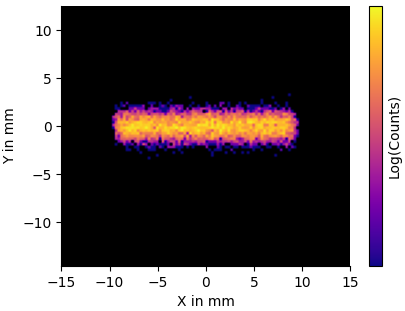
\includegraphics[width=.8\textwidth]{Pos_210.png}
    \caption[Positionsplot des konvergenten Strahls]{Positionsplot des konvergenten Strahls bei einer Flugstrecke von 210 mm.}
    \label{fig:pos_210}
\end{figure}

\begin{figure}[H]
    \centering
    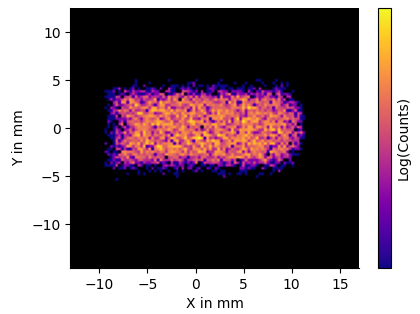
\includegraphics[width=.8\textwidth]{Pos_Forward_Bias.png}
    \caption[Positionsplot mit Vorzugsrichtung der thermischen Bewegung]{Positionsplot mit Vorzugsrichtung der thermischen Bewegung der Ionen. Die Richtungsverteilung der thermischen Bewegung (hier 1/5 eV) ist in einem Kegel um die x-Achse gegeben. Der Öffnungswinkel des Kegels beträgt 110°. Versucht wurde die Verschiebung in x-Richtung des Strahls im Experiment nachzuvollziehen. Allerdings ist kein wesentlicher Unterschied zu Abbildung \ref{fig:sim_pos_kinetic} erkennbar.}
    \label{fig:pos_bias}
\end{figure}   

\begin{landscape}
    \begin{figure}
        \centering
        \hspace{-4cm}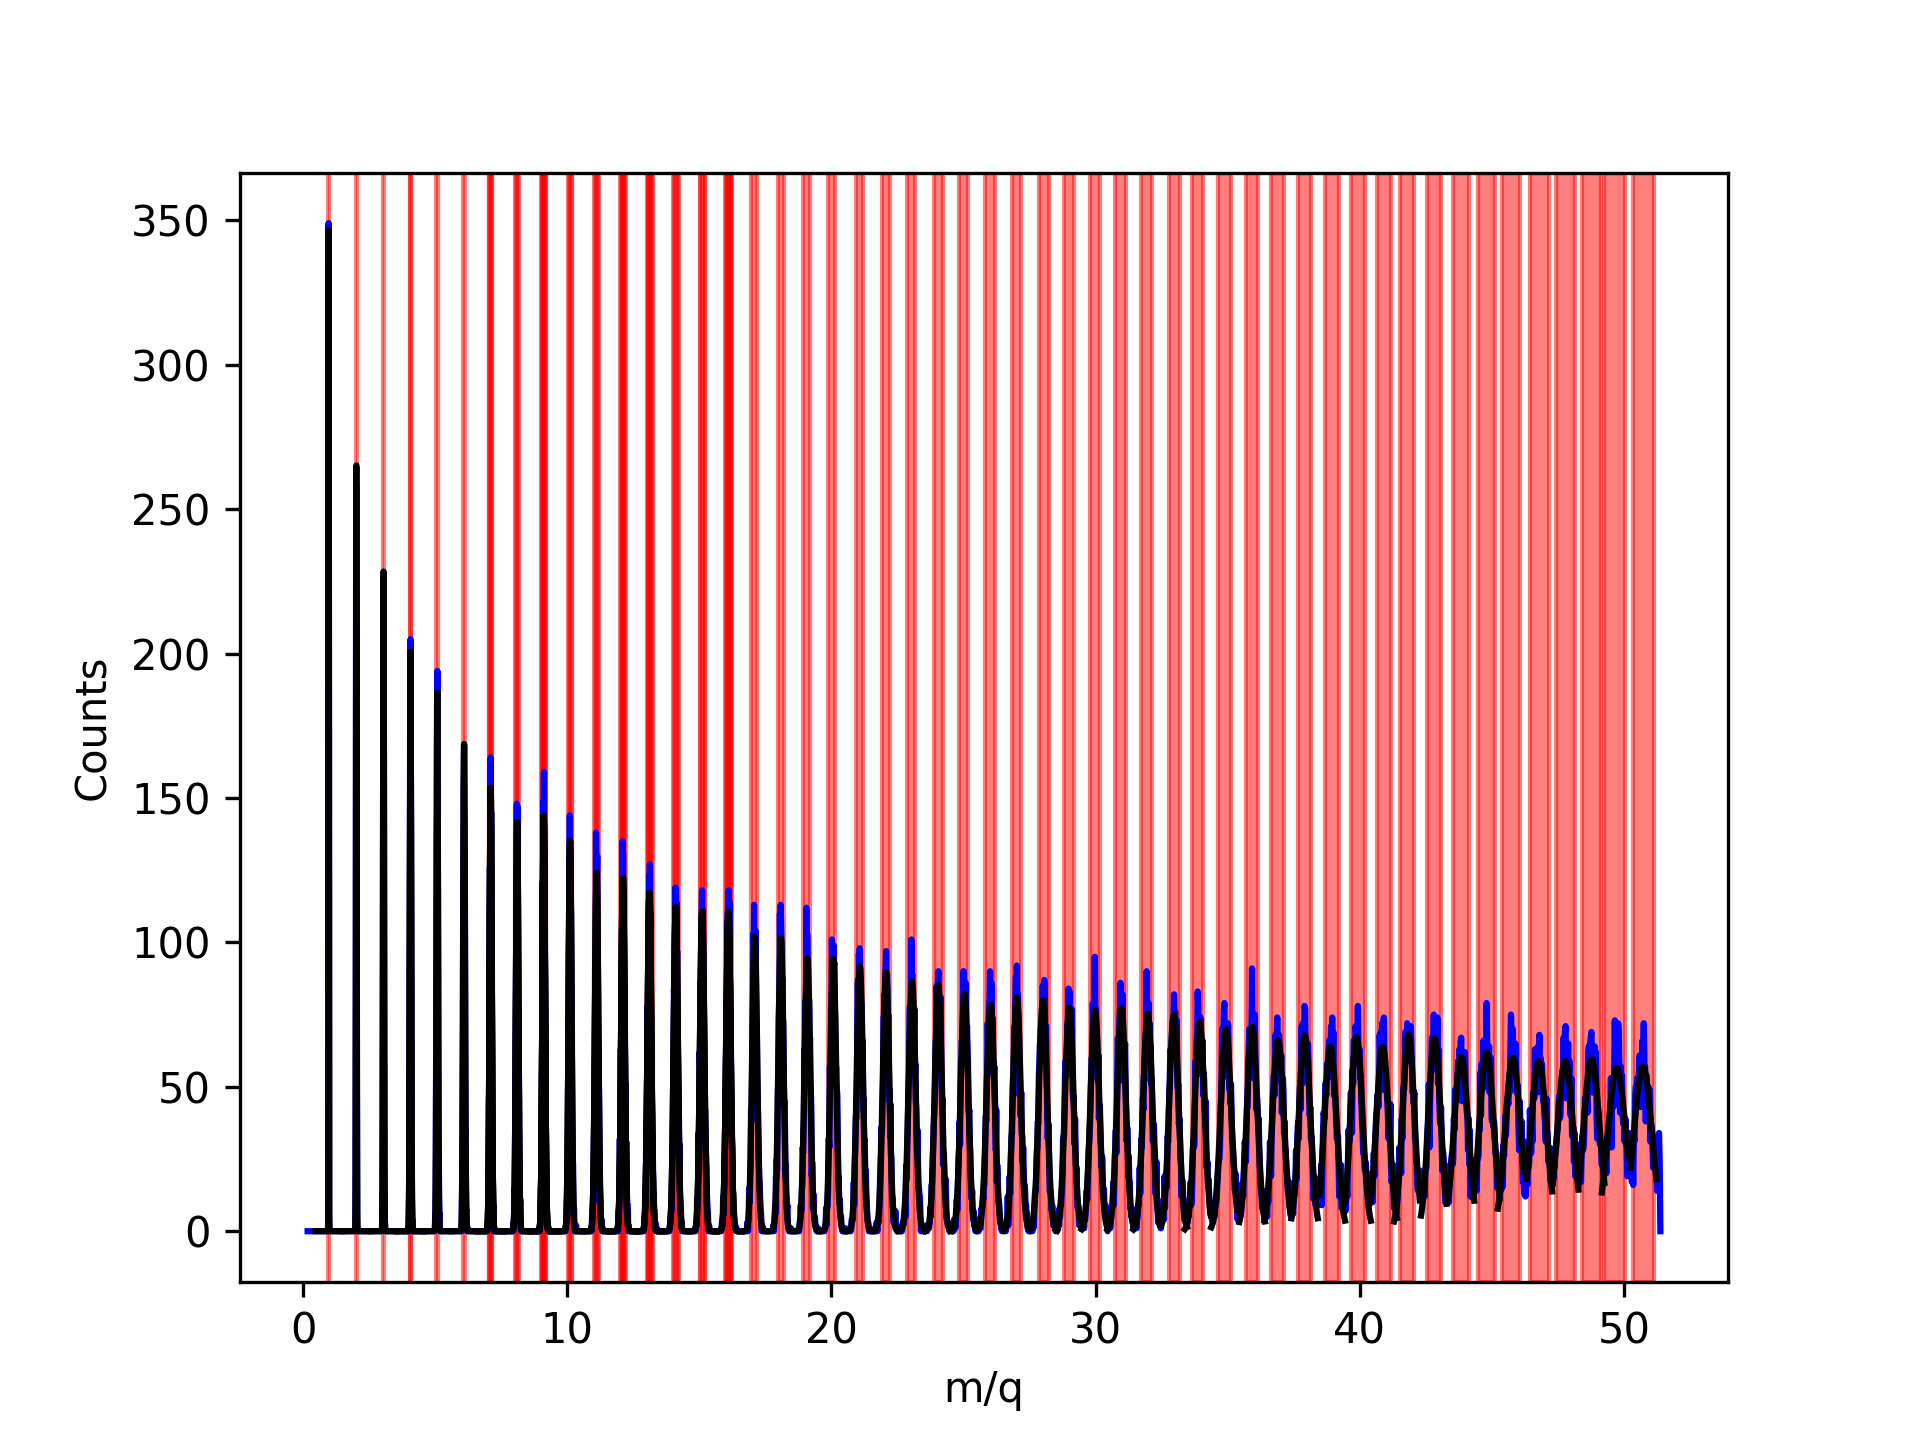
\includegraphics[width=1.3\textwidth]{Resolution_integration.png}
        \caption[Gauß-Fit und Integrationsgrenzen bei Bestimmung der Auflösung]{Gauß-Fit und Integrationsgrenzen bei Bestimmung der Auflösung bei einer Detektordistanz von 410 mm. Der Fit ist in Schwarz dargestellt, die Integrationsgrenzen in Rot und die leicht gefilterten Daten in Blau.}
        \label{fig:integrationsgrenzen}
    \end{figure}
\end{landscape}

\begin{figure}
    \centering
    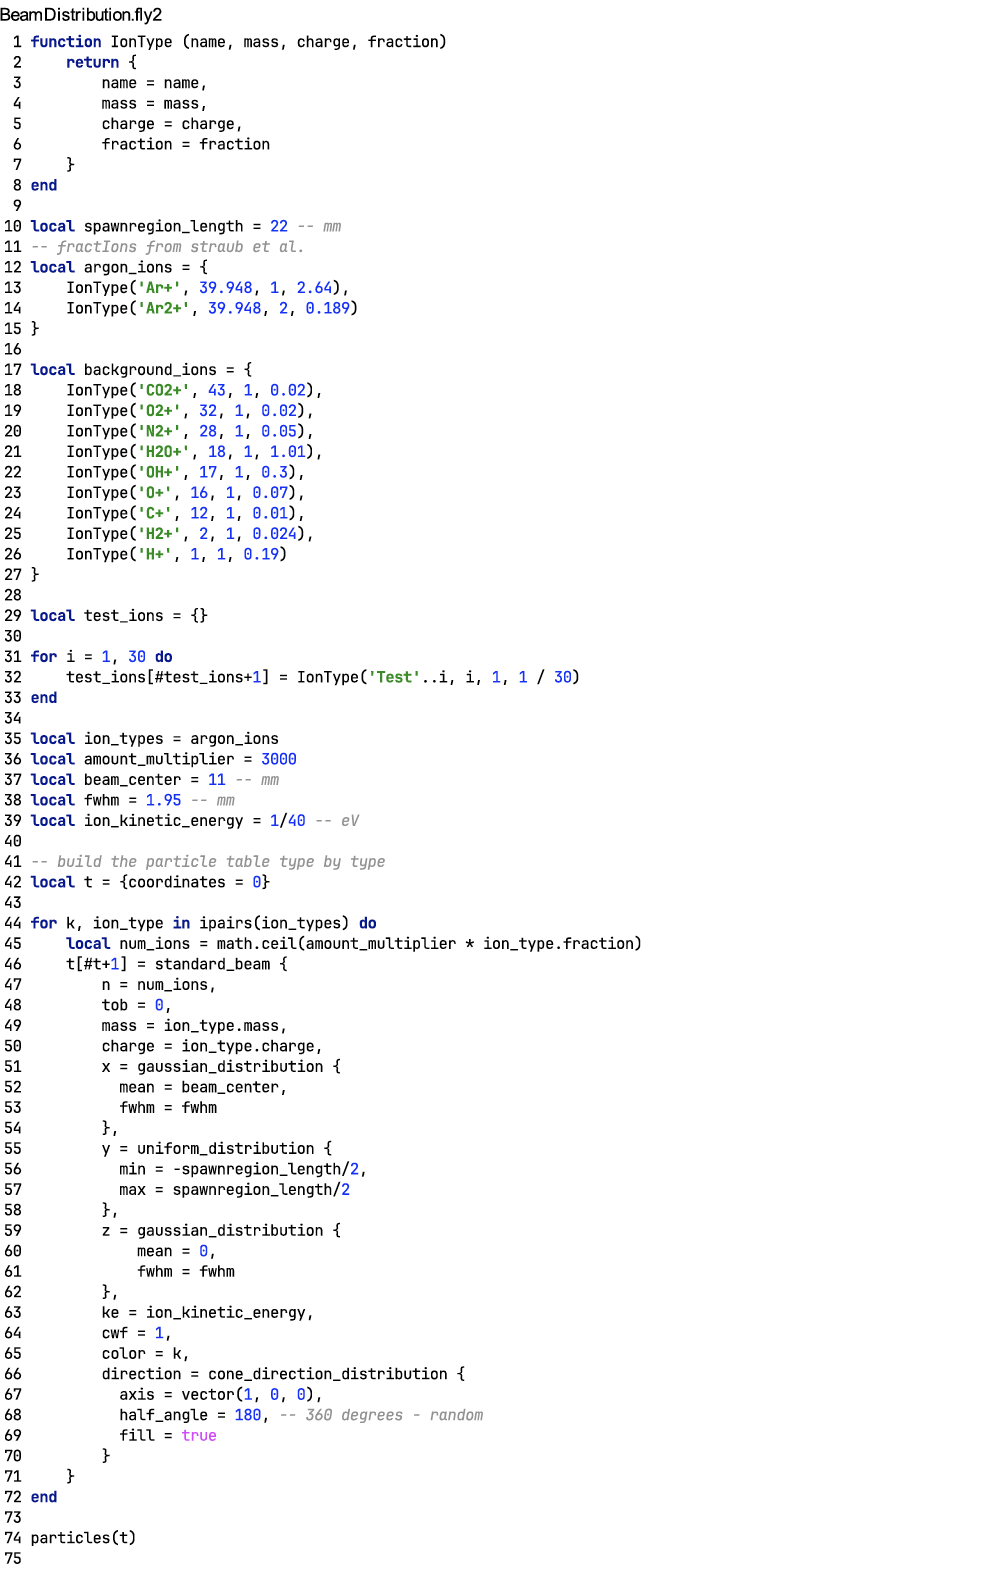
\includegraphics[width=1.05\textwidth]{Fly2.png}
    \caption[Ionenverteilung \textsc{.fly2}-File]{\textsc{.fly2}-File zur Definition der Ionenverteilung in \textsc{Simion} in der Programmiersprache \textsc{Lua}.}
    \label{fly2}
\end{figure}